\section{Introduction}

\begin{figure*}[t]
\centering
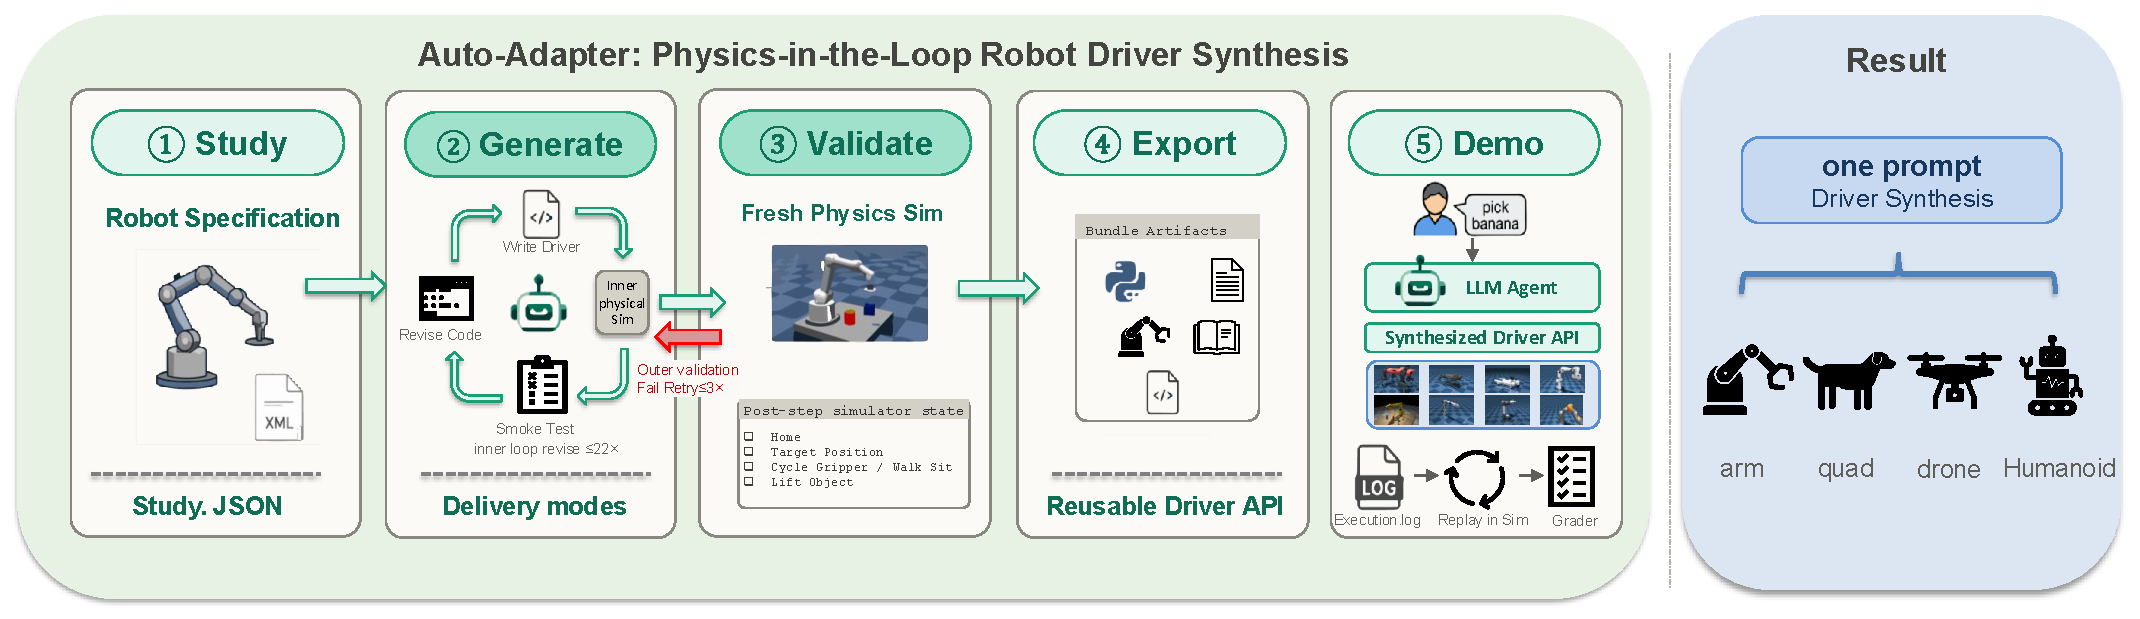
\includegraphics[width=\textwidth]{figures/auto_adapter_overview.pdf}
\caption{The Auto-Adapter pipeline: the agent writes a driver and
verifies it against a physics simulator (inner revise loop, outer
retry), and a downstream agent calls the exported API in Demo
(Algorithm~\ref{alg:generate}).}
\label{fig:pipeline}
\end{figure*}

Tool-using LLM agents have developed an extensive playbook for
\emph{using} tools. ReAct \citep{yao2023react}, Code-as-Policies
\citep{liang2023codeaspolicies}, CodeAct
\citep{wang2024codeact}, Voyager \citep{wang2023voyager}, and
SWE-agent \citep{yang2024sweagent} all assume that the target
system already exposes a tool API: a search endpoint, a Python
interpreter, a hand-authored robot driver. For deployment on a
new target system, the upstream question of how that tool layer
is authored remains open.

\noindent\textbf{Concrete example.}
Consider an SO-ARM101 arm, supplied as an MJCF file (MuJoCo's
XML robot description) listing five joints, six links, a
position-controlled gripper, and joint limits.
A task such as ``move the end-effector (EE) +5\,cm in $X$'' is, for a
tool-using LLM agent, a short sequence of API calls:
\texttt{p $\gets$ get\_ee\_pose(); move\_cartesian(p + [0.05, 0,
0])}. But the agent cannot issue these calls without a Python driver.
The driver translates \texttt{move\_cartesian([x, y, z])} into joint
commands via inverse kinematics (IK), and exposes
\texttt{get\_ee\_pose}, \texttt{gripper\_close}, and the other
primitives the task needs. Today this driver is hand-written per robot.

\noindent\textbf{Three production options.}
Each places the driver outside the LLM's loop. Hand-authoring
the driver and pairing it with Code-as-Policies takes days to
weeks of robotics integration per robot. Finetuning a Vision-Language-Action model such as OpenVLA
\citep{kim2024openvla} requires 10--100 demonstrations and
often fails to generalize beyond its training data.
Protocol-style bridges describe how an LLM talks to a robot but
still require the underlying driver to exist.

\noindent\textbf{Our proposal.}
We hand the driver-authoring step to an LLM agent as well.
Auto-Adapter is a five-phase pipeline (study, generate,
validate, export, demo; Figure~\ref{fig:pipeline}) that reads
MJCF/URDF and emits a self-contained Python driver. The inner
``write code, run, read feedback, revise'' loop is shared with
CodeAct, Reflexion \citep{shinn2023reflexion}, SWE-agent, and
concurrent test-driven controller work \citep{tripathi2026testdriven}.
Our manipulation design has three constraints. First, the output
is a \emph{reusable driver / primitive API} (\texttt{move\_cartesian},
\texttt{get\_ee\_pose}, \texttt{gripper\_close}) for downstream
tool-using agents, not a per-task script. Second, the input is a
formal MJCF/URDF specification, not natural language or a world
image. Third, the verifier reads physics-simulator state after each
step (joint angles, end-effector pose, IK residuals, contact flags),
not text feedback (stdout, judge labels, unit-test pass/fail). The synthesis is scoped: we prescribe the controller class per
morphology (damped-least-squares IK for arms, PD gaits for
quadrupeds). The agent implements, tunes, and validates it rather
than inventing new controllers. We claim no sim-to-real transfer;
the contribution is robotics-oriented software synthesis --- a
physics-verified pipeline for reusable \emph{simulator} drivers
(see Limitations).

\noindent\textbf{Findings.}
The 8-robot onboarding scoreboard (\S\ref{sec:onboarding})
yields structurally validated, smoke-tested drivers in
$7.8 \pm 1.6$ min at $\$2.98 \pm \$0.84$ each (a simulator-side
synthesis cost, not physical bring-up). On SO-101 Reach-and-Pick
our agent and a same-API Code-as-Policies (CaP) baseline both reach 100\%,
while per-skill RL (PPO and Diffusion Policy, DP) needs a separate training
run per skill (\S\ref{sec:capability}). On the full 13-task suite
Auto-Adapter leads the same-API baseline in aggregate (ahead on six
of seven LLMs across five vendors), yet only three \emph{write} their own validated
driver: tool use does not imply tool synthesis
(\S\ref{sec:cap-portability}).

\noindent\textbf{Related work.}
Five threads overlap with ours (expanded in
Appendix~\ref{app:related}). \emph{LLM code-authors}
(Code-as-Policies, Voyager, CodeAct, Eureka \citep{ma2024eureka})
write per-task code over a pre-existing API; we write the API. \emph{LLM tool
creation} (LATM \citep{cai2023latm}, CREATOR
\citep{qian2023creator}) and tool \emph{use} (Toolformer
\citep{schick2023toolformer}, Gorilla \citep{patil2023gorilla})
target \emph{software} tools; we synthesize a \emph{physical-robot}
driver. \emph{Test-driven
controller synthesis} \citep{tripathi2026testdriven} is concurrent
but single-robot; we target 8 robots, emit a reusable driver, and
verify against simulator physics state.
Concurrent agentic-robotics work \citep{enpire2026, capx2026} studies
the same layer from the other side; we synthesize it.
\emph{Robot foundation models} (RT-1/2/X
\citep{brohan2022rt1, brohan2023rt2, openxembodiment2024}, Octo
\citep{octo2024}, OpenVLA, $\pi_0$ \citep{black2024pi0}) often need
per-robot finetuning; we use zero demonstrations. \emph{Protocol
bridges} (RoboNeuron \citep{roboneuron2025}, RCP \citep{rcp2025})
assume a driver exists; we produce it. We
release \textbf{AutoAdapter-Bench}: ten driver artifacts, the
task specification, baseline implementations, and a canonical
results file (anonymized repository linked in the abstract);
every headline number traces to that file.
